%%%%
\section{Fluorescência de Raios X}

Técnica não-destrutiva para análise química elementar 
quantitativa (número atômico Z>10), não exigindo pré-tratamento químico das amostras. 
%TODO: precisa melhorar bem este capítulo todo, colocando a formulação quantitativa para cálculo das concentrações e calibração que fez.

Tipos de fluorescências de Raios X:
\begin{itemize}
  \item Dispersão de Energia
  \item Dispersão de comprimento de onda
  \item Reflexão total
\end{itemize}

Os raios X excitador pode ser gerado em um tubo de raios-x ou por fonte radioativa 
emissoras de raios X.
O rendimento é calculado pelos raios X efetivamente emitidos em relação as 
vacâncias produzidas.
%TODO: de onde surgiu esta vacância? teria que mostrar o processo de excitação se quer discutir o método - colocar figura com átomo de Borhn. Veja a apresentação que fiz sobre xrf, por exemplo. Veja também as referências citadas ali.


Outra forma de excitação usada é por partículas aceleradas 
(elétrons, prótons, íons, partícula alfa e beta negativa).

Amostra espessas apresentam o efeito matriz, ou seja, interações dos 
raios X característicos com os elementos da amostras, causando 
absorção do raios X ou mesmo reforço de raios X.

%%%%
\subsection{Fluorescência de Raios X por dispersão em comprimento de onda}

A dispersão por comprimento de onda é baseada na lei de Bragg.
Usasse critais de difração com distancias interplanares conhecidas.
  
%TODO: citar equação de Barg.

%%%%
\subsection{Fluorescência de Raios X por dispersão em energia}

Os dispersivos em energia usam semicondutor capaz de discriminar energia 
próximas, onde a distinção dos fótons é feita pela amplitude do pulso 
eletrônico produzido no detector, já que os pulsos eletrônicos são
proporcionais às energias dos raios X. 

O detector mais empregado é o detector de silício ativado com lítio, Si(Li).

%%%%
\subsection{Nomenclaturas usadas em Fluorescência de Raios X}
kalfa, kbeta representam transições de fótons nas camnadas dos átomos.
Porém, Algumas transições tem energias tão próximas que é impossível separar.

Transições mais comuns:
\begin{itemize}
  \item $K\alpha$: Transição L para K
  \item $K\beta$: Transição M para K
\end{itemize}

%TODO: Fazer diagrama das transições. Lembrando que há transições proíbidas. 

%%%%
\subsection{Formulação Matemática}

Energia de ligação pode ser aproximada pela teoria atômica de Bohr:
\begin{math}
E = \frac{me^4(Z-b)^2}{8w^2h^2n^2}
\end{math}

\begin{itemize}
  \item E = energia de ligação eletrônica (joules);
  \item m = massa de repouso do elétron = 9,11.10 -31 kilogramas;
  \item e = carga elétrica do elétron = 1,6.10 -19 coulombs;
  \item Z = número atômico do elemento emissor dos raios X;
  \item b = constante de Moseley, com valores iguais a 1 e 7,4, 
        para as camadas K e L, respectivamente;
  \item w = o = permitividade elétrica no vácuo = 8,8534.10 -12 
        coulombs.newton -l .metro -2;
  \item h = constante de Planck = 6,625.10 -34 joules.s;
  \item n = n o quântico principal do nível eletrônico 
        (n = 1 para camada K, n = 2 para camada L, etc.).
\end{itemize}

%%%%
\subsection{Limite de Detecção}

Densidade mínima para haver detecção da espécie. % como determina para XRF?

\begin{figure}[H]
\begin{center}
  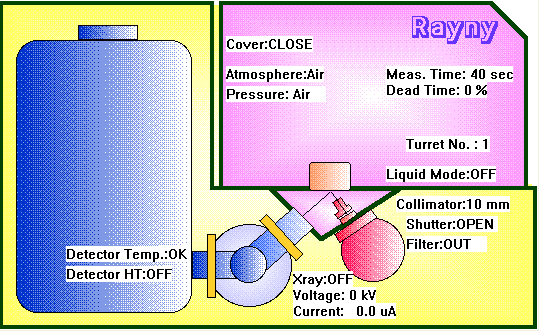
\includegraphics[scale=0.4]{../inputs/images/edx_iag_monitor.png}
  \caption{edx}
\end{center}
\end{figure}



